\documentclass[a4paper,12pt]{article}
\usepackage{graphicx} 
\usepackage{tikz}
\begin{document}

\title{\vspace{-70pt}\begingroup  
    \centering
    \includegraphics[width=0.6\textwidth]{Imaxes/Simbolo_logo_cor transp.png}\\
    \large Grado en Intelixencia Artificial\\
    \large Sistemas Multiaxente\\[0.5em]
    \large \textbf{Práctica 1: Mundo virtual y comportamiento individual}\par 
\endgroup}
\author{Nombre Apellido Apellido2 \\ Nombre Apellido Apellido2 \\ Grupo de clase (martes o viernes)}

\date{}
\maketitle
\vspace{-30pt}


\section*{\large Mundo Virtual}
Resaltad los aspectos más relevantes de vuestro mundo virtual, como decisiones sobre el diseño de habitaciones, pasillos, puertas u otros elementos clave.

Si deseáis participar en la competición al mejor entorno, debéis incluir una imagen de vuestro escenario.
\section*{\large Arquitectura individual}

\begin{center}
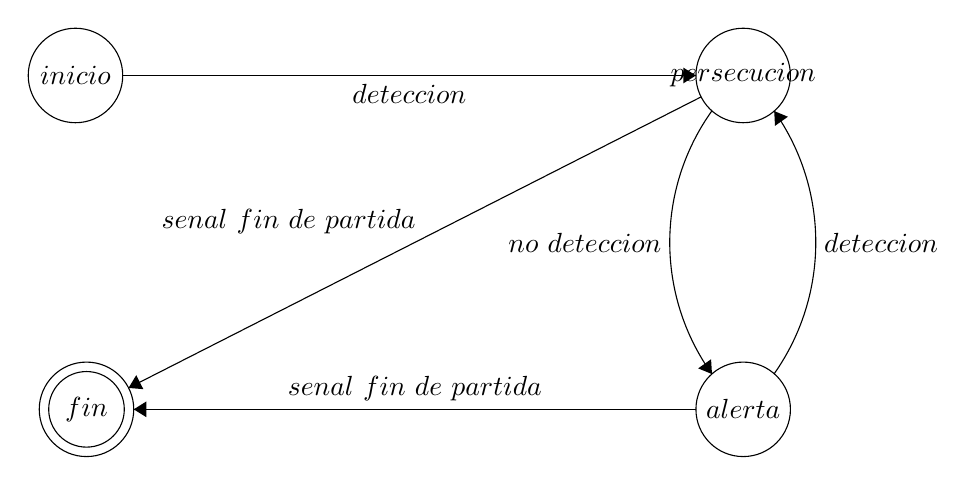
\begin{tikzpicture}[scale=0.2]
\tikzstyle{every node}+=[inner sep=0pt]
\draw [black] (17.8,-28) circle (3);
\draw (17.8,-28) node {$inicio$};
\draw [black] (60.2,-28) circle (3);
\draw (60.2,-28) node {$persecucion$};
\draw [black] (60.2,-49.2) circle (3);
\draw (60.2,-49.2) node {$alerta$};
\draw [black] (18.5,-49.2) circle (3);
\draw (18.5,-49.2) node {$fin$};
\draw [black] (18.5,-49.2) circle (2.4);
\draw [black] (20.8,-28) -- (57.2,-28);
\fill [black] (57.2,-28) -- (56.4,-27.5) -- (56.4,-28.5);
\draw (39,-28.5) node [below] {$deteccion$};
\draw [black] (58.215,-46.958) arc (-144.46201:-215.53799:14.379);
\fill [black] (58.22,-46.96) -- (58.16,-46.02) -- (57.34,-46.6);
\draw (55.04,-38.6) node [left] {$no\mbox{ }deteccion$};
\draw [black] (62.168,-30.258) arc (35.14475:-35.14475:14.492);
\fill [black] (62.17,-30.26) -- (62.22,-31.2) -- (63.04,-30.62);
\draw (65.31,-38.6) node [right] {$deteccion$};
\draw [black] (57.53,-29.36) -- (21.17,-47.84);
\fill [black] (21.17,-47.84) -- (22.11,-47.92) -- (21.66,-47.03);
\draw (31.33,-38.07) node [above] {$senal\mbox{ }fin\mbox{ }de\mbox{ }partida$};
\draw [black] (57.2,-49.2) -- (21.5,-49.2);
\fill [black] (21.5,-49.2) -- (22.3,-49.7) -- (22.3,-48.7);
\draw (39.35,-48.7) node [above] {$senal\mbox{ }fin\mbox{ }de\mbox{ }partida$};
\end{tikzpicture}
\end{center}

Presentad una breve justificación de la arquitectura utilizada en cada uno de vuestros agentes (reactiva, deliberativa, híbrida, BDI, etc.), explicando las razones de vuestra elección.
\section*{\large Sensores}

Describid y justificad la elección de cada uno de los sensores que habéis decidido incluir, explicando su función y relevancia dentro del sistema.
\section*{\large Actuadores}
Describid y justificad la elección de cada uno de los actuadores que habéis decidido incluir, explicando su función y relevancia dentro del sistema.
\end{document}
